\documentclass[a4paper, margin=1cm]{assignment}

\coursetitle{Algorithmen und Datenstrukturen}
\courselabel{AuD}
\exercisesheet{Assignment 1}{Algorithmen und Datenstrukturen}
\student{Moritz Ruge \& Lennard}
\school{Bachelor Informatik}
\university{Freie Universitäten Berlin}
\semester{Sommer Semester 2025}
\date{20 April 2025}
%\usepackage[pdftex]{graphicx}
%\usepackage{subfigure} 
\usepackage[backend=biber,style=numeric,url=true]{biblatex} % für Quellenangaben und Bibliotheken
\usepackage[]{hyperref} % für hyperlinks
\usepackage{array} % für die Tabelle
\usepackage{xcolor} %für Farben bei Text
\addbibresource{ref.bib}  % Add your .bib file here

% Paket für die Baumdiagramdarstellung
\usepackage{tikz}
\usetikzlibrary{trees}


\hypersetup{
    colorlinks=true,
    linkcolor=blue,
    filecolor=magenta,      
    urlcolor=cyan,
    pdftitle={Overleaf Example},
    pdfpagemode=FullScreen,
    }




\begin{document}

% Aufgabe 1 Binäre Suchbäume)
\begin{problemlist}

\pbitem{Induktion und binäre Bäume}
Ein binärer Baum heißt vollständig, falls jeder Knoten entweder null oder zwei Kinder besitzt.
\begin{enumerate}
\item Zeichnen Sie einen binären Suchbaum, der vollständig ist, und einen binären Suchbaum, der nicht vollständig ist.

\item Beweisen Sie durch eine geeignete Induktion: In jedem vollständigen binären Suchbaum ist die Anzahl der Blätter genau um eins größer als die Anzahl der inneren Knoten.

\item Formulieren Sie eine ähnliche Aussage für allgemeine binäre Suchbäume und beweisen Sie sie.
\end{enumerate}

\newpage
\pbitem{Binäre Suchbäume}
\begin{enumerate}
\item Angenommen, wir haben einen binären Suchbaum T , welcher die Zahlen von
1 bis 1000 als Schlüssel speichert. Wir suchen in T nach dem Schlüssel 363.
Bestimmen Sie für jede der folgenden Schlüsselfolgen, ob sie als Folge der
Einträge auf dem Suchpfad nach 363 auftreten kann. Begründen Sie jeweils
Ihre Antwort.


\begin{enumerate}
\item \textbf{2, 252, 401, 398, 330, 344, 397, 363.}

\begin{answer}
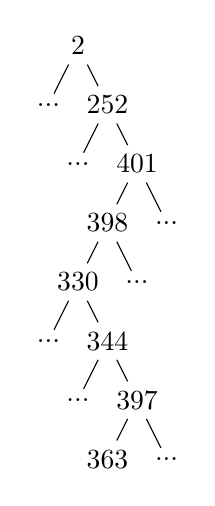
\begin{tikzpicture}[scale=0.5]

\node {2}
	child{node{...}}
	child{ node{252}
		child{node{...}}
		child{node {401}
			child{node{398}
				child{node{330}
					child{node{...}}
					child{node{344}
						child{node{...}}
						child{node{397}
							child{node{363}}
							child{node{...}}}}}
				child{node{...}}}
			child{node{...}}}};
\end{tikzpicture}

\begin{center}
\small
\hspace*{-3cm}
\begin{tabular}{@{} c c l c c @{}}
\toprule
\textbf{Schritt} & \textbf{Aktueller Knoten} & \textbf{Vergleich mit Ziel 363} & \textbf{Nächster Schritt} & \textbf{Intervall für nächsten Knoten} \\
\midrule
1 & 2   & \( 363 > 2 \Rightarrow \) rechts & 252 & \([3, 1000]\) \\
2 & 252 & \( 363 > 252 \Rightarrow \) rechts & 401 & \([253, 1000]\) \\
3 & 401 & \( 363 < 401 \Rightarrow \) links & 398 & \([253, 400]\) \\
4 & 398 & \( 363 < 398 \Rightarrow \) links & 330 & \([253, 397]\) \\
5 & 330 & \( 363 > 330 \Rightarrow \) rechts & 344 & \([331, 397]\) \\
6 & 344 & \( 363 > 344 \Rightarrow \) rechts & 397 & \([345, 397]\) \\
7 & 397 & \( 363 < 397 \Rightarrow \) links & 363 & \([345, 396]\) \\
8 & 363 & Ziel erreicht & — & — \\
\bottomrule
\end{tabular}
\end{center}

\end{answer}

\item \textbf{924, 220, 911, 244, 898, 258, 362, 363.}

\begin{answer}
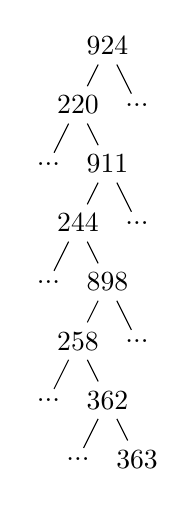
\begin{tikzpicture}[scale=0.5]
\node{924}
	child{node{220}
		child{node{...}}
		child{node{911}
			child{node{244}
				child{node{...}}
				child{node{898}
					child{node{258}
						child{node{...}}
						child{node{362}
							child{node{...}}
							child{node{363}}}}
					child{node{...}}}}
			child{node{...}}}}
	child{node{...}};
\end{tikzpicture}

\begin{center}
\small
\hspace*{-3cm}
\begin{tabular}{@{} c c l c c @{}}
\toprule
\textbf{Schritt} & \textbf{Aktueller Knoten} & \textbf{Vergleich mit Ziel 363} & \textbf{Nächster Schritt} & \textbf{Intervall für nächsten Knoten} \\
\midrule
1 & 924 & \( 363 < 924 \Rightarrow \) links & 220 & \([1, 923]\) \\
2 & 220 & \( 363 > 220 \Rightarrow \) rechts & 911 & \([221, 923]\) \\
3 & 911 & \( 363 < 911 \Rightarrow \) links & 244 & \([221, 910]\) \\
4 & 244 & \( 363 > 244 \Rightarrow \) rechts & 898 & \([245, 910]\) \\
5 & 898 & \( 363 < 898 \Rightarrow \) links & 258 & \([245, 897]\) \\
6 & 258 & \( 363 > 258 \Rightarrow \) rechts & 362 & \([259, 897]\) \\
7 & 362 & \( 363 > 362 \Rightarrow \) rechts & 363 & \([363, 897]\) \\
8 & 363 & Ziel erreicht & — & — \\
\bottomrule
\end{tabular}
\end{center}

\end{answer}


\item \textbf{925, 202, 911, 240, 912, 245, 363.}

\begin{answer}
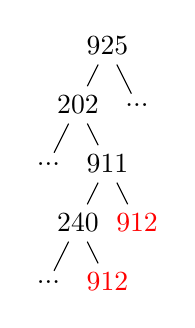
\begin{tikzpicture}[scale=0.5]
\node{925}
	child{node{202}
		child{node{...}}
		child{node{911}
			child{node{240}
				child{node{...}}
				child{node{\textcolor{red}{912}}}}
			child{node{\textcolor{red}{912}}}}}
	child{node{...}};
\end{tikzpicture}

\begin{center}
\small
\hspace*{-3cm}
\begin{tabular}{@{} c c l c c @{}}
\toprule
\textbf{Schritt} & \textbf{Aktueller Knoten} & \textbf{Vergleich mit Ziel 363} & \textbf{Nächster Schritt} & \textbf{Intervall für nächsten Knoten} \\
\midrule
1 & 925 & \( 363 < 925 \Rightarrow \) links & 202 & \([1, 924]\) \\
\bottomrule
\end{tabular}
\end{center}

\end{answer}

\item 2, 399, 387, 219, 266, 382, 381, 278, 363.
\item 935, 278, 347, 621, 299, 392, 358, 363.
\end{enumerate}

\item Sei T ein binärer Baum mit n Knoten, und sei K eine total geordnete Menge
von n Schlüsseln. Zeigen Sie, dass es genau eine Möglichkeit gibt, die Schlüssel
aus K auf die Knoten von T zu verteilen, so dass die binäre Suchbaumeigen-
schaft erfüllt ist.
\end{enumerate}


\pbitem{AVL-Bäume}
\begin{enumerate}
\item Fügen Sie die Schlüssel A, L, G, O, D, T, S, X, Y, Z in dieser Reihenfolge in
einen anfangs leeren AVL-Baum ein. Löschen Sie sodann die Schlüssel Z, A,
L. Zeichnen Sie den Baum nach jedem Einfüge- und Löschvorgang, und zeigen
Sie die Rotationen, welche durchgeführt werden. Annotieren Sie dabei auch
die Knoten mit ihrer jeweiligen Höhe.

\item Beweisen Sie: Beim Einfügen in einen AVL-Baum wird höchstens eine (Einfach-
oder Doppel-)Rotation ausgeführt. Gilt das auch beim Löschen (Begründung)?
\end{enumerate}


	
	
	
\end{problemlist}

%Quellen Reference
%\newpage
%\printbibliography

\end{document}